\chapter{Introduction}
\label{C:intro}

\begin{figure}[t]
\centering
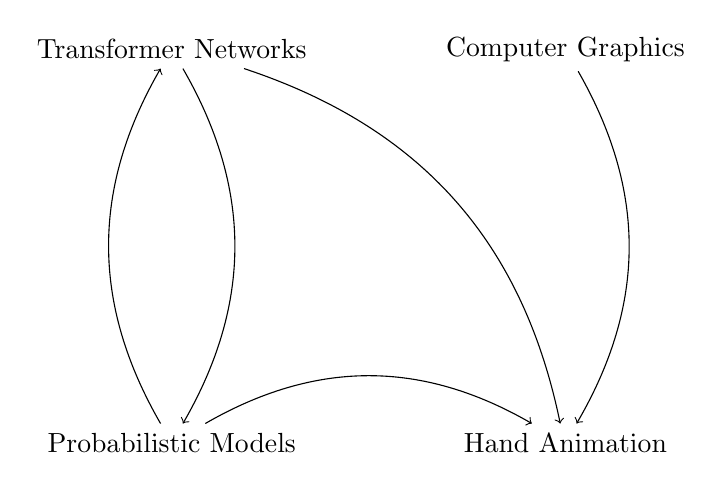
\begin{tikzpicture}
    \tikzstyle{every node}=[node distance=5cm]
    \node (tn) {Transformer Networks};
    \node (pm) [below of=tn] {Probabilistic Models};
    \node (cg) [right of=tn] {Computer Graphics};
    \node (an) [below of=cg] {Hand Animation};

    \draw[->,bend left] (tn) to (pm);
    \draw[->,bend left] (pm) to (tn);
    \draw[->,bend left] (cg) to (an);
    \draw[->,bend left] (pm) to (an);
    \draw[->,bend left] (tn) to (an);
\end{tikzpicture}
\caption[The relationship between the different fields in this thesis]{How learnings and experiments from different fields contribute to each other in this thesis.}
\end{figure}

In this thesis I discuss my learnings and experiments from the past year, which are at the intersection of two areas: Deep Learning and Computer Graphics. There are three main areas of focus:
\begin{enumerate}
    \item I experiment with \textit{transformer} models, and understand them in depth (\Cref{C:transformers}).
    \item I experiment with using Transformer models for Bayesian inference, essentially as Gaussian Processes (\Cref{C:a-o-sampling}).
    \item I create a proof of concept machine learning application for \textit{hand motion prediction}, useful for film and video game production (Chapters \ref{C:angles-joints-hands} and \ref{C:hand-model}).
\end{enumerate}

Although much of my work is summarizing others' research and presenting my learnings, I have two main novel contributions:
\begin{enumerate}
    \item I present experiments with \textit{dynamically-ordered} auto-regressive sampling, which utilises the \textit{permutation-invariance} of the attention operation in transformer models.
    \item I present a proof-of-concept transformer-based generative model for hand motion prediction, which can be used to predict hand motion at arbitrary target frames, and to predict the joints of a hand in any order within that frame.
\end{enumerate}
These contributions involved training neural networks (see \Cref{fig:context}), in particular transformers, on two datasets - MNIST, and a motion capture dataset of hand motion. The results of these experiments are presented in \Cref{C:a-o-sampling} and \Cref{C:hand-model} respectively.


\pgfdeclarelayer{bg}
\pgfsetlayers{bg,main}

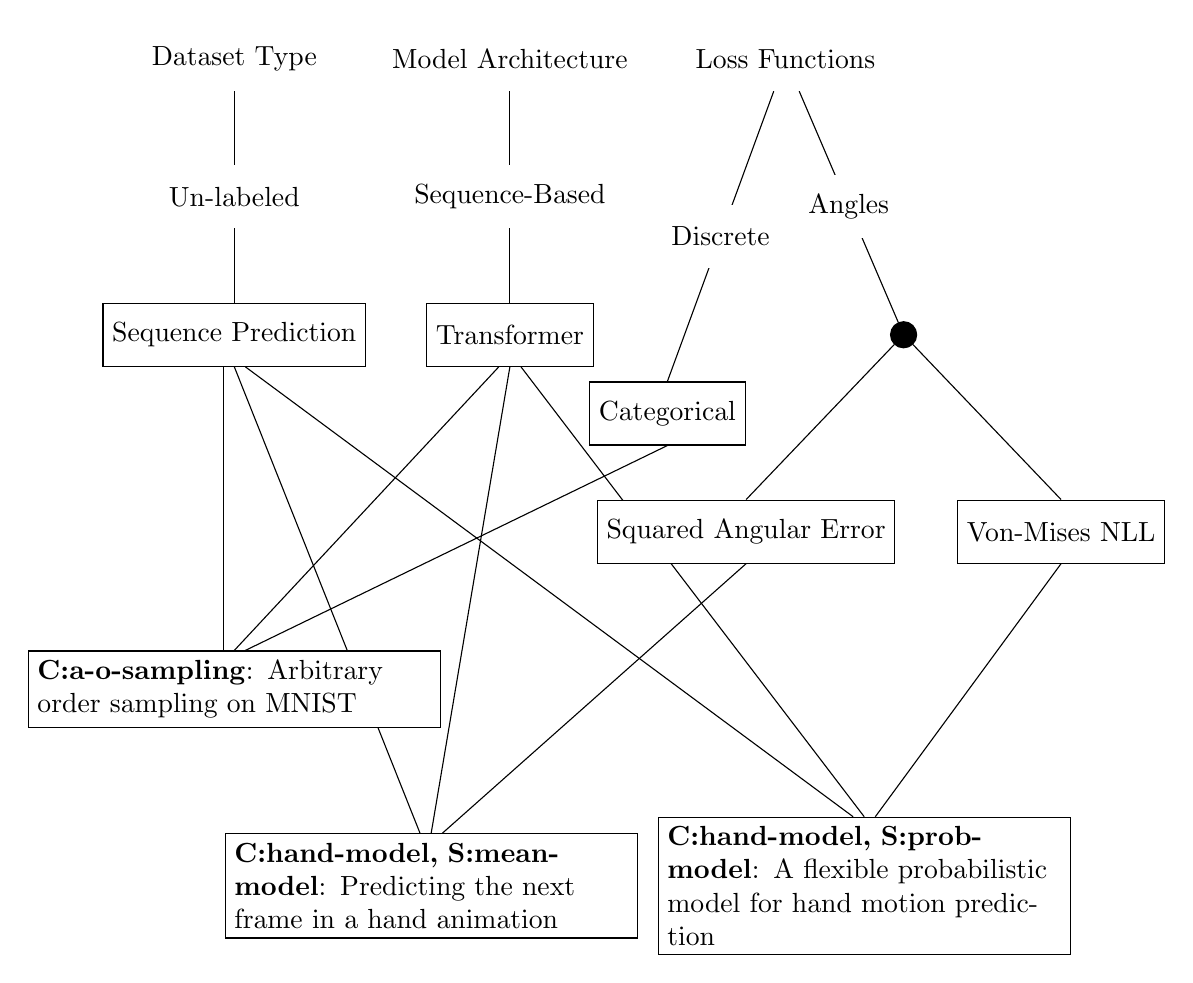
\begin{tikzpicture}
    \tikzstyle{every node}=[node distance=3.5cm,minimum height=0.8cm]

    % dataset type
    \node (datasettype) {Dataset Type};
    \node[draw, below of=datasettype] (seqpred) {Sequence Prediction};
    \draw (datasettype) -- node[fill=white] {Un-labeled} (seqpred);

    % input shape
    \node[right of=datasettype] (seqmodel) {Model Architecture};

    % loss
    \node[right of=seqmodel] (loss) {Loss Functions};

    % angles
    \node[draw,fill=black,minimum height=0.2cm,circle,below of=loss,xshift=1.5cm] (angles) {};
    \draw (loss) -- node[fill=white] {Angles} (angles);

    \node[draw,fill=white,below of=angles,node distance=2.5cm, xshift=-2cm] (amse) {Squared Angular Error};
    \draw (angles) -- (amse.north);

    \node[draw,fill=white,below of=angles,node distance=2.5cm, xshift=2cm] (vonmises) {Von-Mises NLL};
    \draw (angles) -- (vonmises.north);

    \node[draw,fill=white,below of=loss,node distance=4.5cm,xshift=-1.5cm] (cat)  {Categorical};
    \draw (loss) -- node[fill=white] {Discrete} (cat.north);

    % transformer (here because needs to draw above a line)
    \node[draw, below of=seqmodel] (transformer) {Transformer};
    \draw (seqmodel) -- node[fill=white] {Sequence-Based} (transformer);


    % chapter 4: arbitrary order sampling
    \node[draw,fill=white,text width=5cm] (chapter4) at (0,-8cm) {\textbf{\Cref{C:a-o-sampling}}: Arbitrary order sampling on MNIST};

    % chapter 6.2: transformer for hand pose prediction
    \node[draw,fill=white,text width=5cm] (chapter62) at (2.5cm,-10.5cm) {\textbf{\Cref{C:hand-model}, \Cref{S:mean-model}}: Predicting the next frame in a hand animation};

    % chapter 6.3: probabilistic model for hand pose prediction
    \node[draw,fill=white,text width=5cm] (chapter63) at (8cm,-10.5cm) {\textbf{\Cref{C:hand-model}, \Cref{S:prob-model}}: A flexible probabilistic model for hand motion prediction};

    \begin{pgfonlayer}{bg}
        \draw ([xshift=-4pt]seqpred.south) -- ([xshift=-4pt]chapter4.north);
        \draw ([xshift=-4pt]transformer.south) -- (chapter4.north);
        \draw (cat.south) -- ([xshift=4pt]chapter4.north);

        \draw (seqpred.south) -- ([xshift=-4pt]chapter62.north);
        \draw (transformer.south) -- (chapter62.north);
        \draw (amse.south) -- ([xshift=4pt]chapter62.north);

        \draw ([xshift=4pt]seqpred.south) -- ([xshift=-4pt]chapter63.north);
        \draw ([xshift=4pt]transformer.south) -- (chapter63.north);
        \draw (vonmises.south) -- ([xshift=4pt]chapter63.north);
    \end{pgfonlayer}
\end{tikzpicture}


In the rest of this chapter, I will discuss the motivation for this thesis, and previous work that relates to it.

\section{Motivation}
\label{s:motivation}
The problem domain I focused on -- hand motion prediction -- is a sequence prediction problem, which are  the general kind of task that transformer models are used on. To this end, I hoped to find that these two motivations would feed back into each other as I worked -- the application providing direction for the more general / theoretical research, and the insights gained from the more general research contributing back to better solutions for the problem domain.

\subsection{Why focus on hand motion?}
\label{ss:why-hand-motion}

Whenever a moving virtual character appears in an animated film or a video game, someone had to spend the time to specify the angles of all the joints. Fortunately is not necessary to lay out every single frame, because animation tools used for both games and film production make use of interpolation techniques between key-frames, but artists must still specify many joints, over many key-frames, over many different kinds of animation.

In order to fully animate a character, an animator needs to appropriately animate all moving parts of that character. We can divide these into three groups, each involving a similar amount of work:
\begin{itemize}
    \item Facial animation -- animating the muscles of the face when a character talks or otherwise makes facial expressions.
    \item Hand animation -- animating the fingers and wrists when a character makes gestures or manipulates objects.
    \item Body animation (also simply called character animation) -- animating the rest of the body, e.g. the legs, arms, neck and spine when a character walks, dances, etc.
\end{itemize}

Of these, the face and body are often the most noticeable, and most of the time recieve the most attention from the audience. However, the hands are also very important, and are often the most difficult to animate.

\TODO{Examples of problematic hand animation.}

\subsection{Why focus on transformers?}
\label{ss:why-transformers}


\section{Previous Work}
